\documentclass{article} 
\usepackage{listings}
\usepackage{graphicx}
\usepackage{subfig}
\usepackage{multirow}
\usepackage{float}
\usepackage{algorithm}
\usepackage{algpseudocode}
\usepackage{amsmath}

\newenvironment{algocolor}{%
   \setlength{\parindent}{0pt}
   \itshape
   \color{blue}
}{}

\lstset
{ %Formatting for code in appendix
    language=Python,
    %basicstyle=\footnotesize,
    numbers=left,
    stepnumber=1,
    showstringspaces=true,
    tabsize=4,
    breaklines=true,
    breakatwhitespace=false,
}

\title{AI 534 IA4 Report}
\author{Rishab Balasubramanian}
\date{}

\begin{document}
\maketitle

\textbf{1.}a. The split for the root is \textit{``odor=n"}, with an information gain of $0.535$. Next the feature used to split the tree is \textit{``bruises?=f"}, with a gain of almost $0.4$. The next split is with the feature \textit{``spore-print-color=r"} with a gain of approximately $0.103$.\\

b. Fig.\ref{fig:DT} shows the effect of the maximum depth $d_{max}$ on the efficiency of Decision Trees. We see that the accuracies increase with the increase in depth of the tree. At $d_{max} = 6$, we get a $100\%$ accuracy on both the training and validation data. In this case we do not observe overfitting due to the relatively simple dataset, and as a result both the training and validation accuracies increase with the depth upto a maximum accuracy of $100\%$.

\begin{figure}[H]
    \centering{{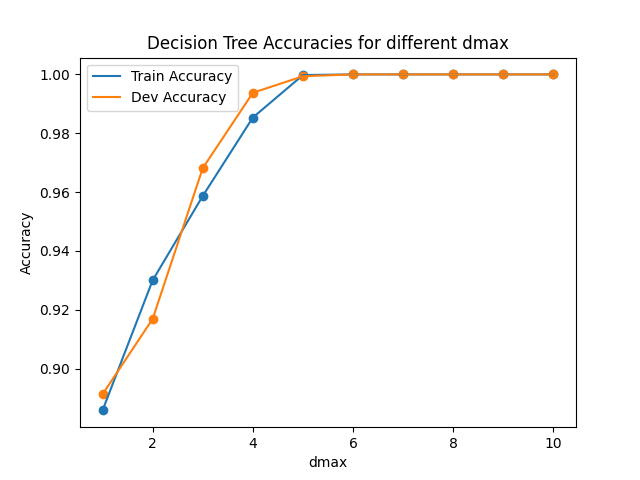
\includegraphics[width=\textwidth]{DT.png} }}\\
\caption{Accuracy of Decision Trees with different depths}
    \label{fig:DT}%
\end{figure}

\textbf{2.}a. Fig.\ref{fig:RF_train} and Fig.\ref{fig:RF_valid} shows the training  and validation accuracies of the random forest at different depths. Note that in Fig.\ref{fig:RF_train}c, the accuracies of $m=25$ and $m=50$ are almost equal to $100\%$. We see that at $dmax = 1$, the maximum training accuracy reached is $94\%$, and the maximum validation accuracy reached is $92\%$. This shows that the model is underfitting as we know that a single decision tree is able to reach an accuracy of $100\%$. Similarly at $dmax = 2$, the training and validation accuracies are below $98\%$, and again we see that the model underfits. We get prety good accuracies with an ensemble size of$50$ trees, and at this point our model is almost perfectly fitting. We see that at $dmax = 5$, the model has a very high accuracy of $99\%$ on both the training and validation datasets for $25$ and $50$ trees, and as a result we can say that the model fits well. For $5$ and $10$ trees, the model performs poorly, and we can conclude it underfits Because the validation accurcies are also equally high, we can say that the random forest does not overfit either, and this is a good learned model. In all cases the validation and training accuracies are comparable and so we can say that the random forest does not overfit.

\begin{figure}[H]
    \centering
    \subfloat[\centering Depth = 1]{{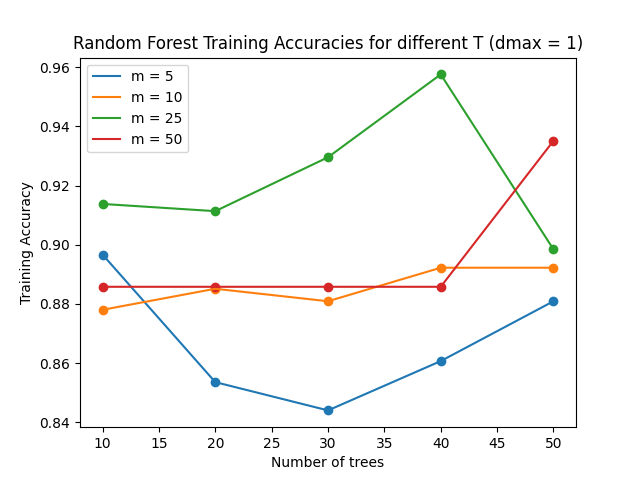
\includegraphics[width=0.33\textwidth, height=4cm]{RF_training_dmax=1.png} }}
    \subfloat[\centering Depth = 2]{{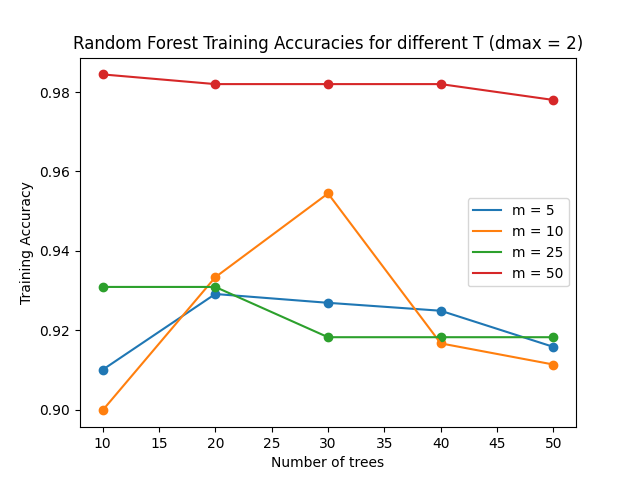
\includegraphics[width=0.33\textwidth, height=4cm]{RF_training_dmax=2.png} }}
    \subfloat[\centering Depth = 5]{{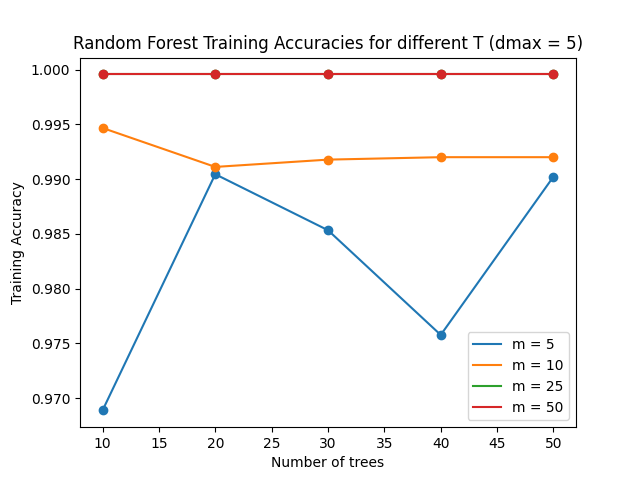
\includegraphics[width=0.33\textwidth, height=4cm]{RF_training_dmax=5.png} }}\\
\caption{Random Forest Training Accuracies}
    \label{fig:RF_train}%
\end{figure}

\begin{figure}[H]
    \centering
    \subfloat[\centering Depth = 1]{{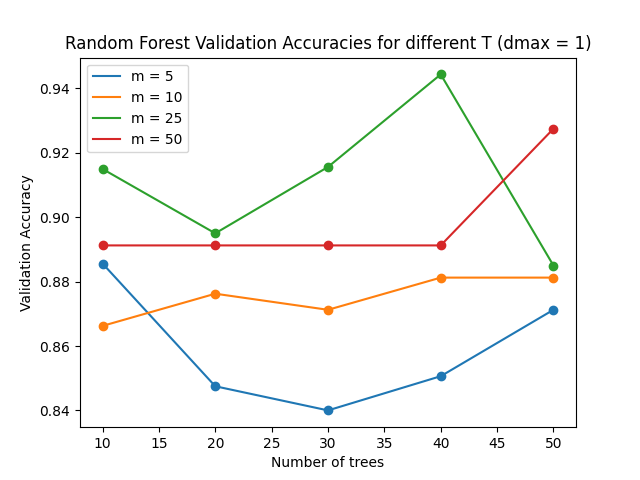
\includegraphics[width=0.33\textwidth, height=4cm]{RF_valid_dmax=1.png} }}
    \subfloat[\centering Depth = 2]{{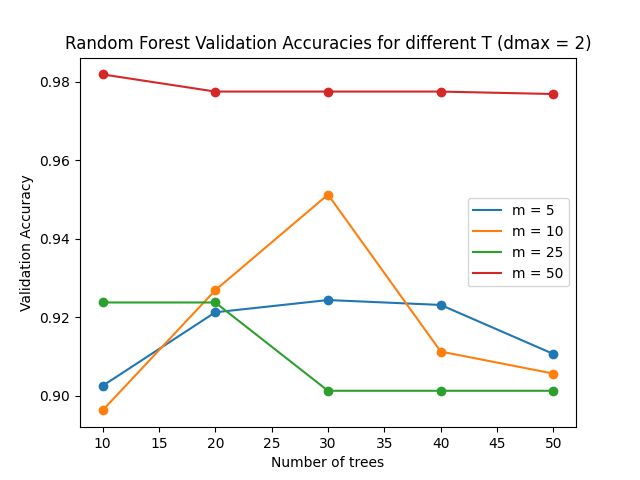
\includegraphics[width=0.33\textwidth, height=4cm]{RF_valid_dmax=2.png} }}
    \subfloat[\centering Depth = 5]{{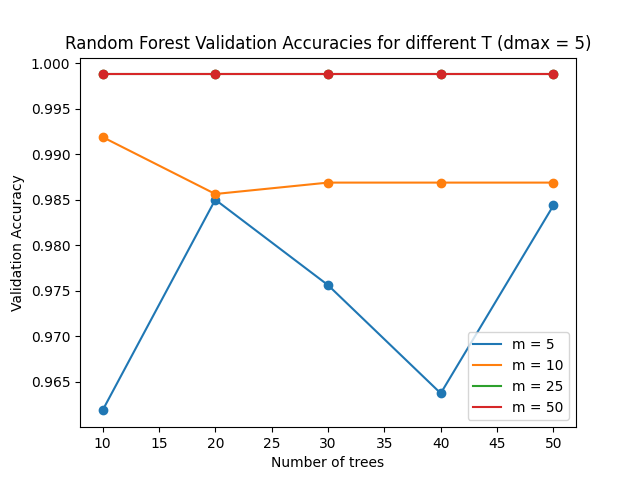
\includegraphics[width=0.33\textwidth, height=4cm]{RF_valid_dmax=5.png} }}\\
\caption{Random Forest Validation Accuracies}
    \label{fig:RF_valid}%
\end{figure}

b. At $dmax=1$, the model has a high bias and low variance. This is because the training and validation accuracies are almost equal (showing that the model has low variance), but both accuracies are quite low (indicating the model is not able to generalize to the data, thus indicating high bias). At $dmax=2$, with $50$ trees, the model still has low variance, as the training and validation accuracies are almost equal, and bias lower than at $dmax=1$. With a lower ensemble size, the random forest still underfits as we can see the training and validation accuracy are quite low. This is because the training and validation accuracies are significantly higher than at $dmax=1$, indicating the model is able to learn better. Finally, at $dmax=5$, we see that both training and validation accuracies are almost equal, and are both close to $100\%$ with $25$ and $50$ trees. This shows the model has learnt a good generalization of the data, that it can extend to the validation set as well. Thus at $dmax=5$, we have low bias and low variance. We see that the Random Forest model performs significantly worse than the Decision Trees. This may be because of the relatively simple nature of the dataset. It may also be caused by the very small subsample of features (atmost $50$ out of $118$ available features, which is lesser than $50\%$ of the features). This could be the reason for the poor performance of the algorithm. We also observe that with a lower ensemble size the random forest almost always performs poorly. Using a larger subset of features, a larger number of trees or Bagged Decision Trees instead of Random Forest would be better in this case. As we know that even short trees give relatively good performance, a larger subsample of parameters might improve the performance of the random forest.\\

\textbf{3.}a. Fig.\ref{fig:Adaboost} shows the training and validation accuracies for the Adaboosted trees with varying ensemble size For $dmax=1$, we see that when the ensemble size is small, the model underfits a little, as we can see that the training accuracy is lower than the validation accuracy and both of them are lesser than $100\%$ which is acheivable using Decision Trees. For $dmax=2$, and $dmax=5$, we see that the model perfectly fits as it is able to learn a representation that acheives close to $100\%$ accuracy on both training and validation datasets.\\

\begin{figure}[H]
    \centering
    \subfloat[\centering Depth = 1]{{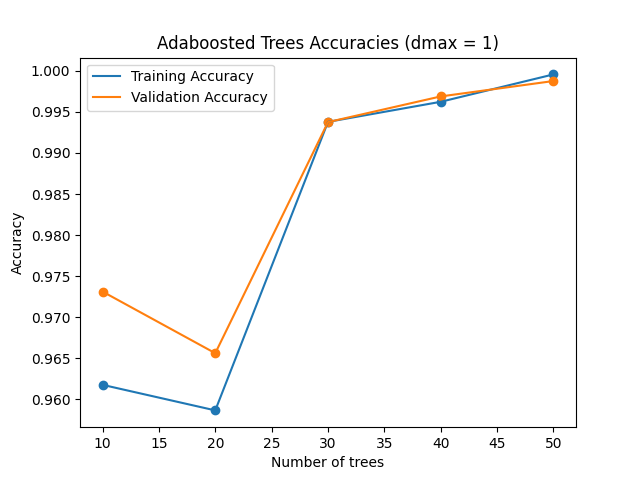
\includegraphics[width=0.33\textwidth, height=4cm]{Adaboost_dmax=1.png} }}
    \subfloat[\centering Depth = 2]{{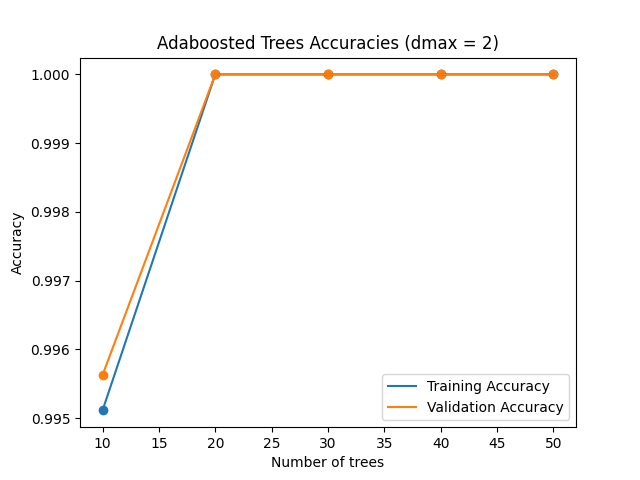
\includegraphics[width=0.33\textwidth, height=4cm]{Adaboost_dmax=2.png} }}
    \subfloat[\centering Depth = 5]{{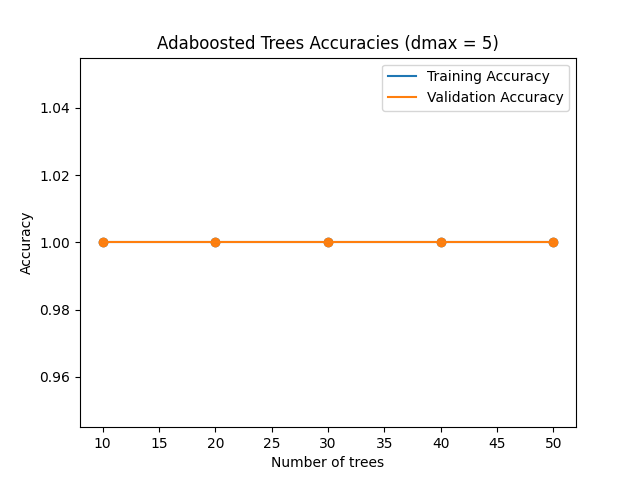
\includegraphics[width=0.33\textwidth, height=4cm]{Adaboost_dmax=5.png} }}\\
\caption{Random Forest Validation Accuracies}
    \label{fig:Adaboost}%
\end{figure}

b. As discussed before, we see that at $dmax=1$, the model underfits a little, as the training accuracies and validation accuracies are comparable to each other but lower than $100\%$. Thus the model posseses some bias at lower ensemble size (upto around $20$ trees) at $dmax=1$. Beyond this the model fits perfectly, similar to $dmax=2$, and $dmax=5$. Thus at a higher ensemble size for $dmax=1$, and for all versions in $dmax=2$ and $dmax=5$, the model has low bias and high accuracy. As the adaboosted trees fit the data very well, it does not need any changes. Given the simplicity of the data, the adaboosted tree algorithm worked significantly well.

\end{document}